\documentclass[a4paper]{report}
\usepackage{ctex}
\usepackage{geometry}
\geometry{left=3.17cm,right=3.17cm,top=2.54cm,bottom=2.54cm}

\title{分布式调度器设计文档}
\author{共轭空间开源组}
\begin{document}
\maketitle
\tableofcontents
\chapter{简介} % (fold)
\label{sec:简介}
chin 是一个支持定时\&依赖的轻量级分布式调度系统,相比于Linkin开源的azkaban调度系统,它占用的内存更少;相比于Airbnb开源的AirFlow调度系统,它占用的CPU更少;相比于Luigi以及上述两者,它管理界面更友好。

由于是轻量级系统,因此它很容易移植到ARM系列的处理器上(事实上我正是为了解决上述系统无法在ARM架构的机器下正常工作而写的这个调度系统)。它可以执行所有的linux命令,包括但并不只局限于
\begin{itemize}
	\item command
	\item shell
	\item python
	\item java
	\item etc...
\end{itemize}

我们的后端语言选择golang,因为golang部署容易,不需要额外的依赖。 前端框架选择vue,数据库选择mysql,客户端选择android。






\chapter{使用指南} % (fold)

\section{如何安装} % (fold)
\subsection{下载} % (fold)
\subsection{安装} % (fold)
\subsection{配置} % (fold)


\section{如何启动} % (fold)
启动命令: 

./chin args

其中,args可选的参数为
\begin{itemize}
	\item master: 启动 master 服务
	\item worker: 启动 worker 服务
	\item webserver: 启动 web 服务
	\item build\_db: 清空数据表后重新建表,并新建root用户
	\item clean\_db: 清空表中的所有数据
	\item mock\_db: mock数据
\end{itemize}



\chapter{设计详情} % (fold)


\section{任务生命周期} % (fold)
\subsection{简介} % (fold)
\begin{figure}[htbp]
\centering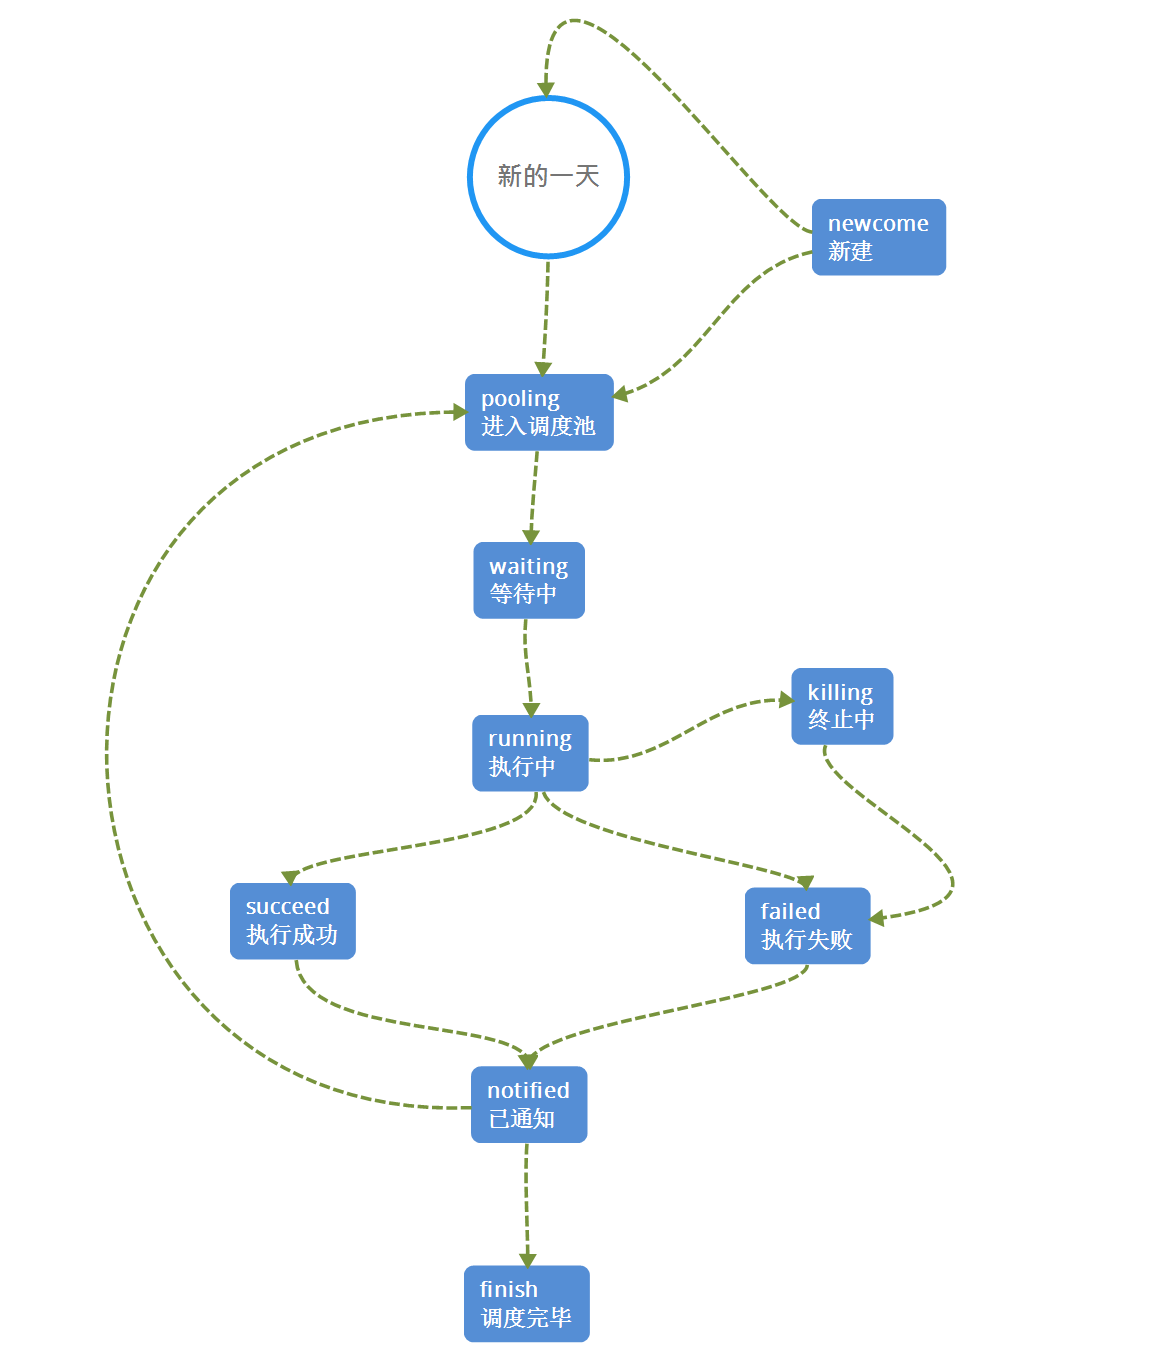
\includegraphics[width=3.5in]{生命周期.png}
\caption{任务生命周期}
\end{figure}
任务的生命周期共有八个状态:新建(newcome)、进入调度池(pooling)、等待中(waiting)、执行中(running)、执行成功(succeed)、执行失败(failed)、终止中(killing)、已通知(notified)、调度完毕(finish)。其中,newcome是一个逻辑上存在的状态,在物理上并不存在。各状态的转换流程如图所示。

\subsection{状态周期} % (fold)
\subsubsection{新建(newcome)} % (fold)
\begin{figure}[htbp]
\centering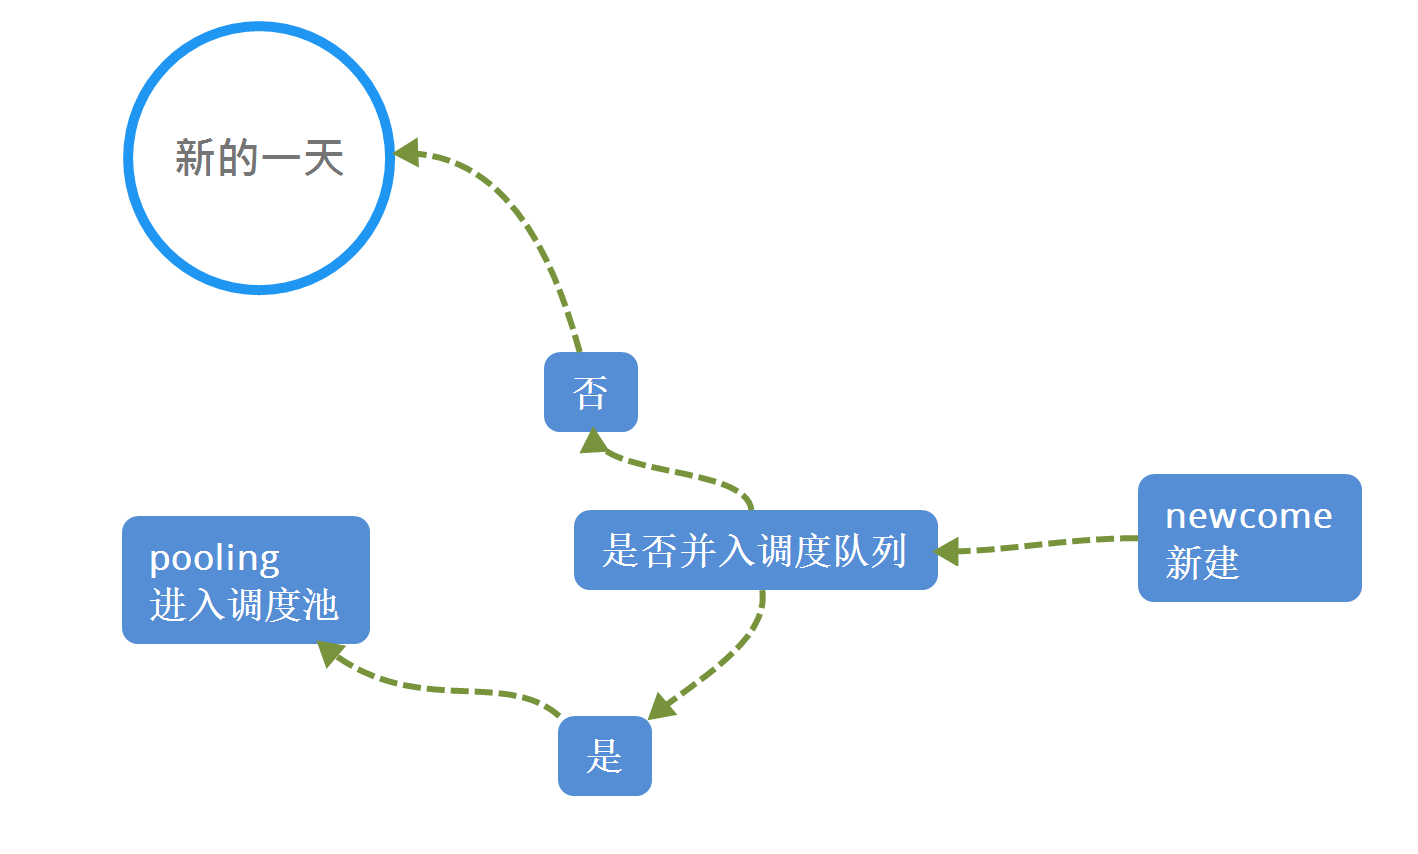
\includegraphics[width=3.5in]{newcome.png}
\caption{newcome状态}
\end{figure}
newcome只是逻辑上存在的状态,在任务新建时,其状态为newcome状态。处于newcome状态下的任务会有两种行为,如果用户点击并入队列,那么就会新建一个任务实例放进调度队列,进入到pooling状态,否则,会一直处于newcome状态一直到往后一天进入例行的调度。

\subsubsection{进入调度池(pooling)} % (fold)
\begin{figure}[htbp]
\centering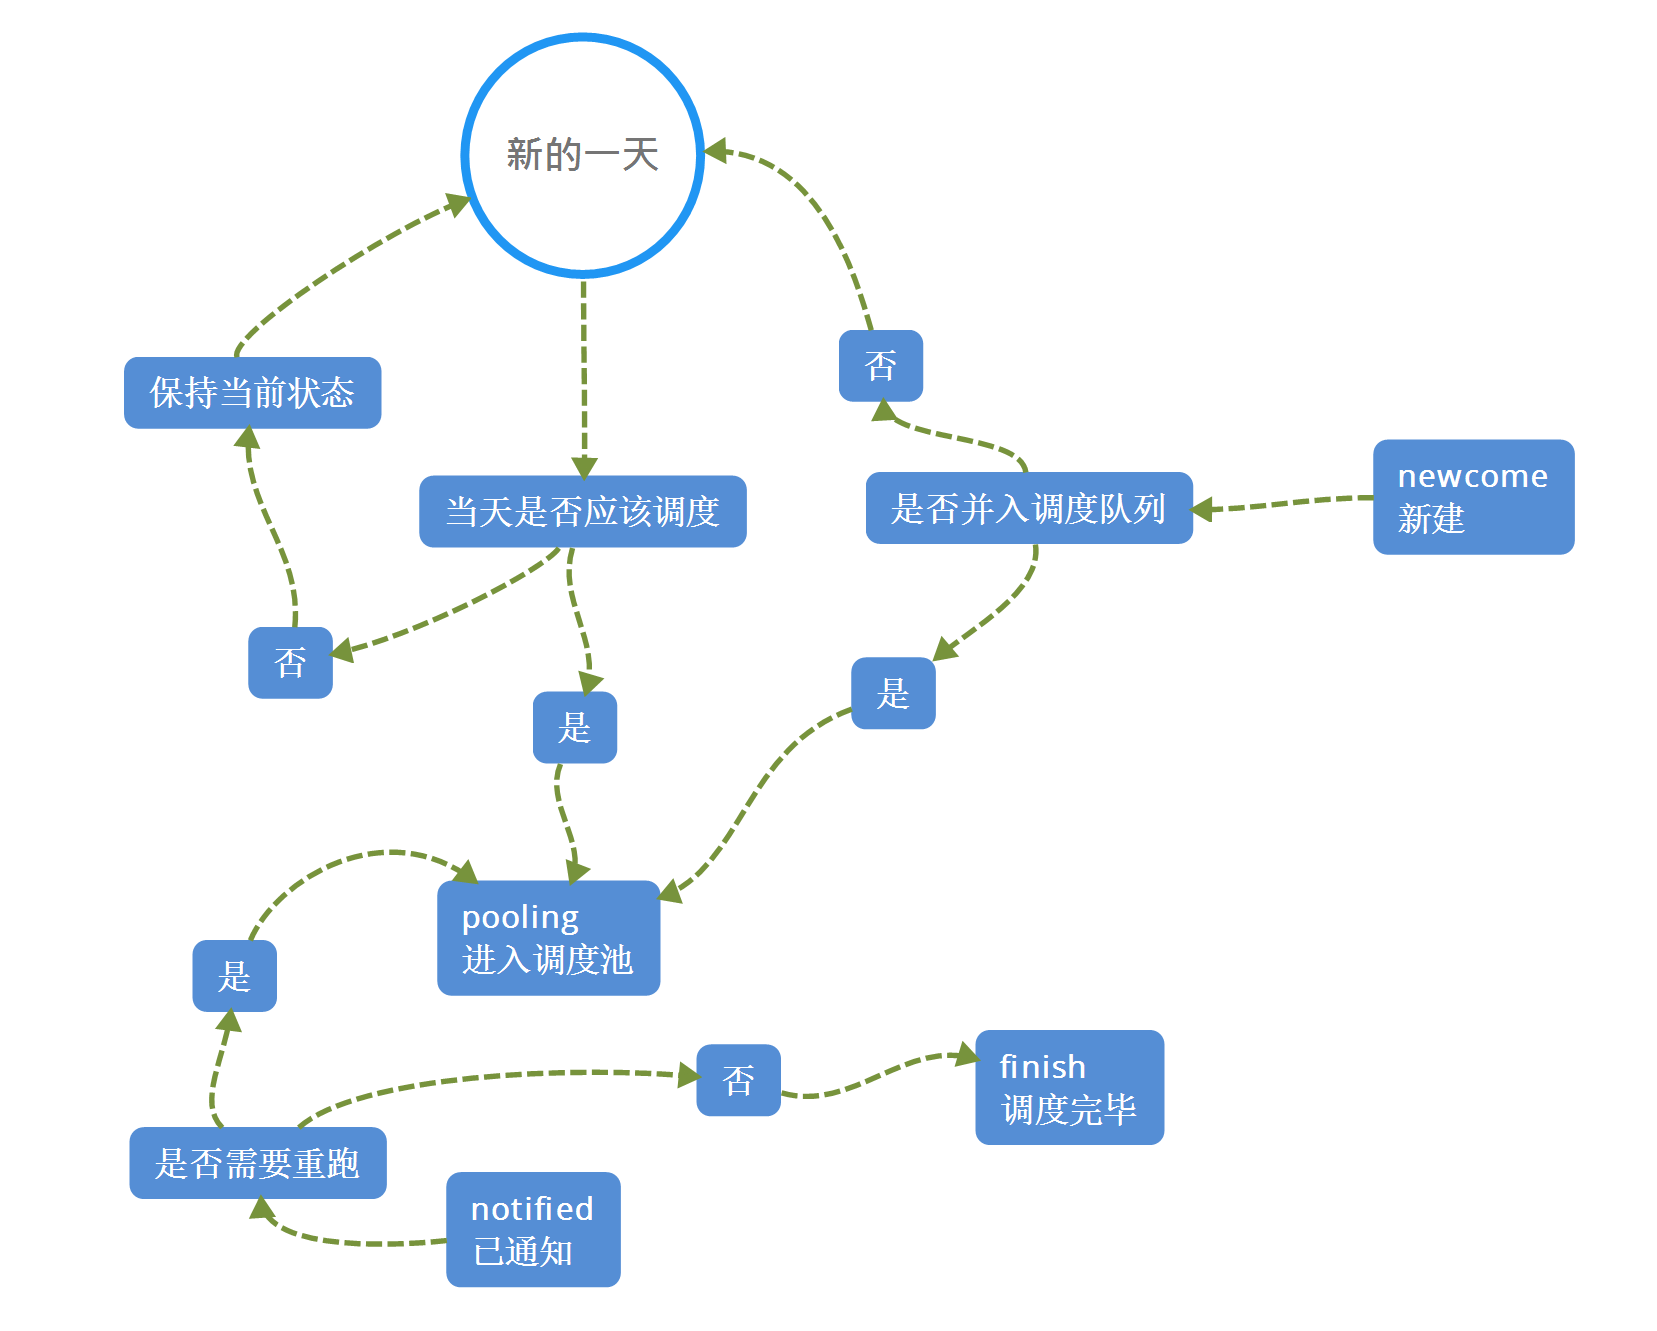
\includegraphics[width=3.5in]{pooling.png}
\caption{pooling状态}
\end{figure}
有三种情况会使得任务实例进入 pooling 状态:第一种,正如 newcome 状态里所说的,如果一个任务新建后,用户点击并入队列,那么就会新建一个任务实例,并进入到 pooling 状态。第二种,当新的一天来临,如果这个任务的 valid = true,即例行调度为真,并且,当天日期符合调度周期和调度格式,那么会新建一个任务实例,状态为 pooling。第三种情况,如果某个任务实例处于 notified 状态,并且需要重跑,那么状态会更新为 pooling。


\subsubsection{等待执行(waiting)} % (fold)
\begin{figure}[htbp]
\centering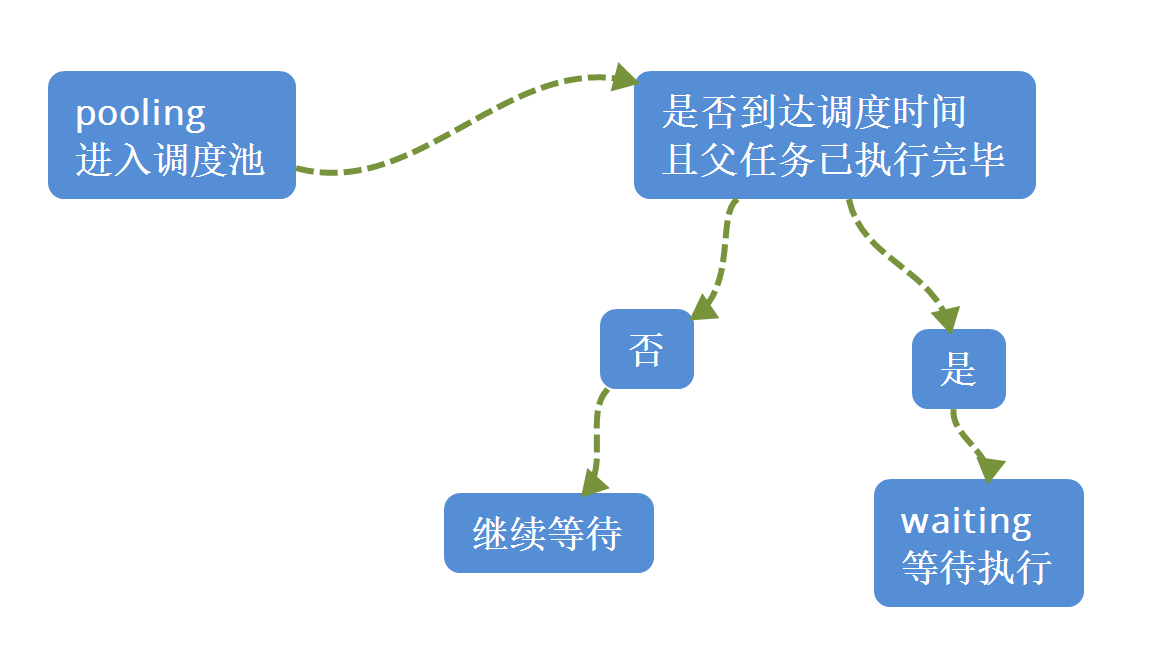
\includegraphics[width=3.5in]{waiting.png}
\caption{waiting状态}
\end{figure}
当某个任务实例处于 pooling 状态时,一旦它依赖的父任务执行完毕,并且到达它的调度时间,则会进入到 waiting 状态,等待调度器给它分配执行机器。

\subsubsection{执行中(running)} % (fold)
\begin{figure}[htbp]
\centering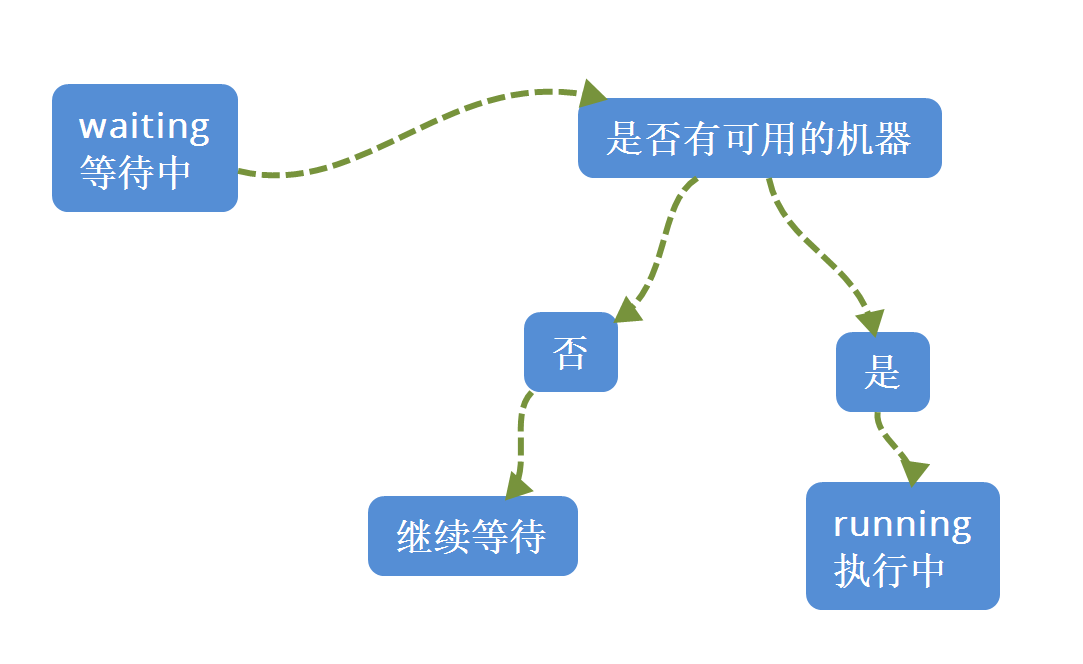
\includegraphics[width=3.5in]{running.png}
\caption{running状态}
\end{figure}
当某个任务实例处于 waiting 状态时,一旦有可用的机器,则开始执行任务,并将状态更新为 running。



\subsubsection{终止中(killing)} % (fold)
当任务实例处于 running 状态时,用户手动点击终止执行操作,则会使任务进入 killing 状态,等待后台杀死进程。


\subsubsection{执行成功/失败(succeed/failed)} % (fold)
任务执行完毕后,根据任务的执行结果,将状态更新为成功或失败,由于被杀死的任务其返回值也是失败,所以状态也是失败。
\begin{figure}[htbp]
\centering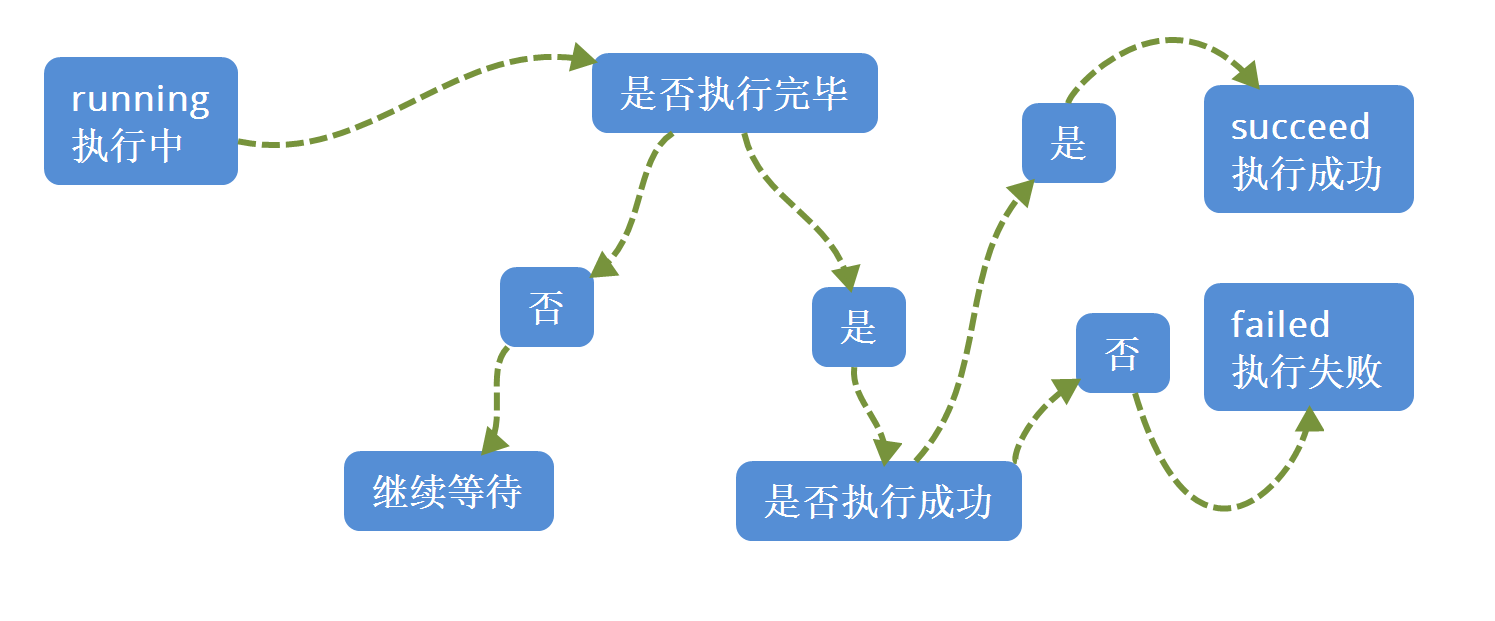
\includegraphics[width=3.5in]{succeed.png}
\caption{succeed/failed状态}
\end{figure}

\subsubsection{已通知(notified)} % (fold)
执行成功或执行失败的任务,判断其是否需要通知,如果需要,则将信息通过邮件发送给用户,然后进入notified状态;如果不需要,则直接进入notified状态
\begin{figure}[htbp]
\centering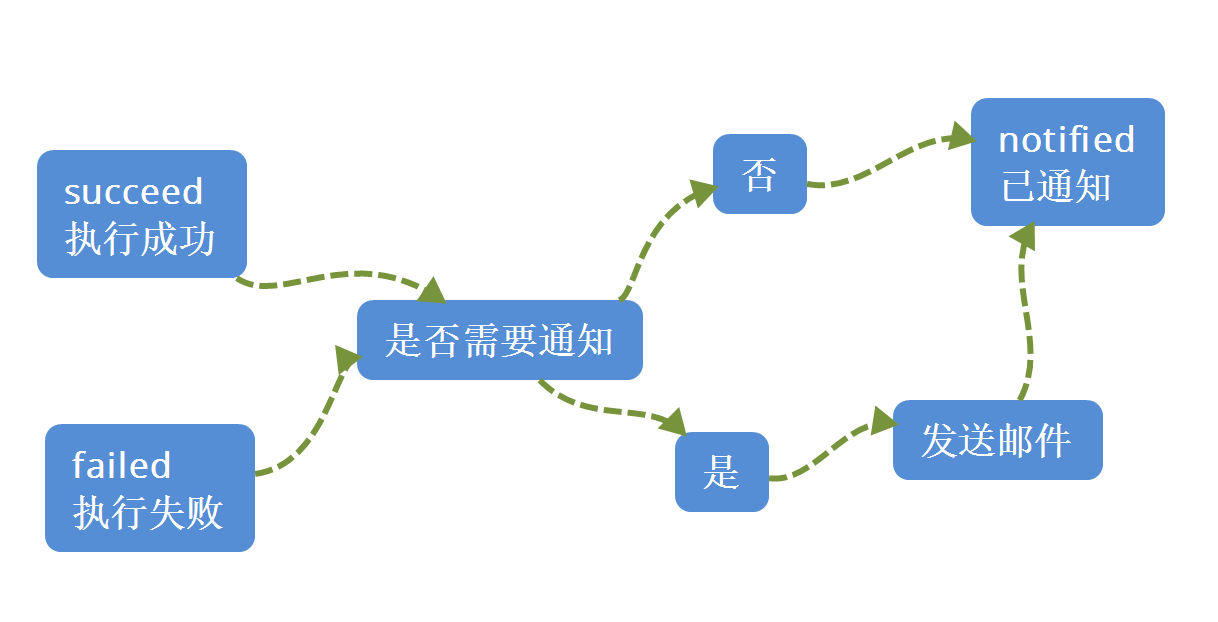
\includegraphics[width=3.5in]{notified.png}
\caption{notified状态}\label{fig:1}
\end{figure}


\subsubsection{调度完毕(finish)} % (fold)
通知完毕后的任务进入调度完毕状态。



\subsection{特殊事件} % (fold)
\subsubsection{调度器重启} % (fold)
调度器重启后,会检查有没有老任务(即非当天新建的任务)没有被创建实例,如果有,则会创建实例。

\subsubsection{worker重启} % (fold)
worker重启后,会把属于自己并且状态为 running 的任务实例其状态置为 failed

\subsubsection{并入队列} % (fold)
如果一个任务在当天本不应该执行,比如,某个任务调度周期为每周三,而今天是周五,我希望这个任务今天也调度,那么我点击并入队列,则会新建一个实例,进入到 pooling 状态

\subsubsection{立即执行}
如果某个任务不存在实例,则新建一个实例,然后跳过 pooling 状态,直接进入 waiting 状态,如果存在实例,则直接将实例置为 waiting 状态。

\subsubsection{置为成功} % (fold)
立即将一个任务实例的状态设置为成功,如果一个任务位于running状态,则需要手动 killing 后才能强制成功


\subsubsection{凌晨跨天时当天任务没有执行} % (fold)
如果跨天时,某个任务实例的状态为 pooling 或 waiting,那么调度器将直接把任务状态设置为failed



\section{系统组件} % (fold)
\subsection{master}
用于分配任务、跟踪任务执行情况、worker判活等。它要是挂了,client还能正常工作,但不不再会有任务调度

\subsection{worker}
用于执行任务。它要是挂了,master会报警,如果任务可以在别的机器上执行,那么master会把任务分配到别的机器上。

\subsection{db}
用于存储元数据和系统日志。整个系统中,MySQL是核心,所有的组件都围绕MySQL进行通讯,如果MySQL挂了,那所有组件都不能工作了,我们称之为:真·药丸。

\subsection{client}
用户终端,两个版本,PC端和Android端,用于可视化的对任务进行增删改查。









\section{负载均衡} % (fold)
\subsection{均衡策略} % (fold)
\subsection{worker判活} % (fold)



\section{数据表设计} % (fold)

\subsection{任务表} % (fold)
\begin{tabular}{|c|c|c|}
	\hline \multicolumn{3}{|c|}{task}\\
	\hline task\_id           &bigint    &任务ID\\
	\hline task\_name         &string    &任务名\\
	\hline command            &string    &任务执行命令\\
	\hline father\_id         &string    &父任务ID,以逗号间隔,-> task.task\_id\\
	\hline valid      	      &tinyint   &是否例行调度,0-不调度 1-调度\\
	\hline machine\_pool      &string    &可执行机器ID,以逗号间隔,-> machine.machine\_id\\
	\hline owner\_id   	      &string    &任务所属者ID, -> user.user\_id\\
	\hline schedule\_type     &string    &调度周期\\
	\hline schedule\_format   &string    &调度格式\\
	\hline create\_time   	  &string    &创建时间\\
	\hline update\_time       &string    &更新时间\\
	\hline 
\end{tabular}

\subsection{实例表} % (fold)
\begin{tabular}{|c|c|c|}
	\hline \multicolumn{3}{|c|}{task}\\
	\hline instance\_id       &bigint    &实例ID\\
	\hline task\_id           &string    &任务ID, -> task.task\_id\\
	\hline status   	      &string    &任务实例所在的生命周期状态\\
	\hline create\_time   	  &string    &创建时间\\
	\hline update\_time       &string    &更新时间\\
	\hline 
\end{tabular}

\subsection{执行日志表} % (fold)
\begin{tabular}{|c|c|c|}
	\hline \multicolumn{3}{|c|}{log}\\
	\hline log\_id            &bigint    &日志ID\\
	\hline instance\_id       &bigint    &实例ID, -> instance.instanct\_id\\
	\hline machine\_id        &bigint    &执行机器ID, -> machine.machine\_id\\
	\hline output         	  &string    &日志输出\\
	\hline create\_time   	  &string    &创建时间\\
	\hline update\_time       &string    &更新时间\\
	\hline 
\end{tabular}


\subsection{操作日志表} % (fold)
\begin{tabular}{|c|c|c|}
	\hline \multicolumn{3}{|c|}{action}\\
	\hline action\_id         &bigint    &操作日志ID\\
	\hline user\_id           &bigint    &操作者ID, -> user.user\_id\\
	\hline content         	  &string    &操作内容\\
	\hline create\_time   	  &string    &创建时间\\
	\hline update\_time       &string    &更新时间\\
	\hline 
\end{tabular}



\subsection{用户表} % (fold)
\begin{tabular}{|c|c|c|}
	\hline \multicolumn{3}{|c|}{user}\\
	\hline user\_id           &bigint    &用户ID\\
	\hline user\_name         &string    &用户名\\
	\hline password           &string    &登陆密码\\
	\hline email         	  &string    &用户邮箱\\
	\hline create\_time   	  &string    &创建时间\\
	\hline update\_time       &string    &更新时间\\
	\hline 
\end{tabular}



\subsection{机器表} % (fold)
\begin{tabular}{|c|c|c|}
	\hline \multicolumn{3}{|c|}{machine}\\
	\hline machine\_id           &bigint    &机器ID\\
	\hline machine\_name         &string    &机器名\\
	\hline ip                    &string    &机器IP\\
	\hline mac         	         &string    &机器MAC地址\\
	\hline cpu\_load         	 &int    	&CPU负载\\
	\hline menory\_load          &int    	&内存负载\\
	\hline alive         	 	 &int    	&是否活着\\
	\hline create\_time   	     &string    &创建时间\\
	\hline update\_time          &string    &更新时间\\
	\hline 
\end{tabular}







\chapter{API} % (fold)
\label{sec:api}
\section{任务} % (fold)

\subsection{新增任务}
\subsubsection{Method \& URL} % (fold)
POST /api/task/new 

\subsubsection{请求JSON字段}
\begin{itemize}
	\item \textbf{token:} string, required, 用户登陆后获取到的session
	\item \textbf{user\_id:} bigint, required, 用户ID
	\item \textbf{task\_name:} string, required, 任务名
	\item \textbf{command:} string, required, 任务执行命令
	\item \textbf{father\_id:} array[bigint], required, 任务的父任务
	\item \textbf{valid:} \{true, false\}, required, 任务是否例行调度
	\item \textbf{machine\_pool:} array[bigint], required, 可执行该任务的机器列表
	\item \textbf{schedule\_type:} \{'once', 'day', 'week', 'month'\}, required, 调度周期
	\item \textbf{schedule\_format:} string, required, 调度格式
\end{itemize}

\subsubsection{返回JSON字段}
\begin{itemize}
	\item \textbf{status:} \{'SUCCEED', 'FAILED'\}, 返回状态
	\item \textbf{info:} string, 返回信息
\end{itemize}


\subsection{删除任务} % (fold)
\subsubsection{Method \& URL} % (fold)
POST /api/task/delete, 本操作只能由任务所属者或root用户操作

\subsubsection{请求JSON字段}
\begin{itemize}
	\item \textbf{token:} string, required, 用户登陆后获取到的session
	\item \textbf{user\_id:} bigint, required, 用户ID
	\item \textbf{task\_id:} bigint, required, 任务ID
\end{itemize}

\subsubsection{返回JSON字段}
\begin{itemize}
	\item \textbf{status:} \{'SUCCEED', 'FAILED'\}, 返回状态
	\item \textbf{info:} string, 返回信息
\end{itemize}



\subsection{修改任务} % (fold)
\subsubsection{Method \& URL} % (fold)
POST /api/task/modify, 本操作只能由任务所属者或root用户操作

\subsubsection{请求JSON字段}
\begin{itemize}
	\item \textbf{token:} string, required, 用户登陆后获取到的session
	\item \textbf{user\_id:} bigint, required, 用户ID
	\item \textbf{task\_name:} string, required, 任务名
	\item \textbf{command:} string, required, 任务执行命令
	\item \textbf{father\_id:} array[bigint], required, 任务的父任务
	\item \textbf{valid:} \{true, false\}, required, 任务是否例行调度
	\item \textbf{machine\_pool:} array[bigint], required, 可执行该任务的机器列表
	\item \textbf{schedule\_type:} \{'once', 'day', 'week', 'month'\}, required, 调度周期
	\item \textbf{schedule\_format:} string, required, 调度格式	
\end{itemize}

\subsubsection{返回JSON字段}
\begin{itemize}
	\item \textbf{status:} \{'SUCCEED', 'FAILED'\}, 返回状态
	\item \textbf{info:} string, 返回信息
\end{itemize}



\subsection{查询任务} % (fold)
\subsubsection{Method \& URL} % (fold)
POST /api/task/query

\subsubsection{请求JSON字段}
\begin{itemize}
	\item \textbf{token:} string, required, 用户登陆后获取到的session
	\item \textbf{user\_id:} bigint, required, 用户ID
	\item \textbf{batch:} \{true, false\} required, 是否分页查询
	\item \textbf{task\_id:} bigint, optional, 任务ID,当batch=false时必选
	\item \textbf{page:} int, optional, 页数,当batch=true时必选
	\item \textbf{page\_size:} int, optional, 页大小,当batch=true时必选
\end{itemize}

\subsubsection{返回JSON字段}
\begin{itemize}
	\item \textbf{status:} \{'SUCCEED', 'FAILED'\}, 返回状态
	\item \textbf{info:} string, 返回信息
	\item \textbf{data:} \{array[json], json\}, 当batch=true时返回任务信息的json, 当batch=false时返回任务信息json的array
\end{itemize}






\section{执行日志} % (fold)
\subsection{查询执行日志} % (fold)
\subsubsection{Method \& URL} % (fold)
POST /api/log/query

\subsubsection{请求JSON字段}
\begin{itemize}
	\item \textbf{token:} string, required, 用户登陆后获取到的session
	\item \textbf{user\_id:} bigint, required, 用户ID
	\item \textbf{batch:} \{true, false\}, required, 是否分页查询
	\item \textbf{given\_task:} \{true, false\}, required, 是否只查询某个任务的日志
	\item \textbf{task\_id:} bigint, optional, 任务ID,当given\_task=true时必选
	\item \textbf{log\_id:} bigint, optional, 日志ID,当given\_task=false并且batch=false时必选
	\item \textbf{column:} array[string], optional, 查询的字段,若不提供则查询所有的字段
	\item \textbf{page:} int, optional, 页数,当batch=true时必选
	\item \textbf{page\_size:} int, optional, 页大小,当batch=true时必选
\end{itemize}

\subsubsection{返回JSON字段}
\begin{itemize}
	\item \textbf{status:} \{'SUCCEED', 'FAILED'\}, 返回状态
	\item \textbf{info:} string, 返回信息
	\item \textbf{data:} \{array[json], json\}, 当batch=true时返回日志json的array, 当batch=false时返回任务信息json
\end{itemize}




\section{操作日志} % (fold)
\subsection{查询操作日志} % (fold)
\subsubsection{Method \& URL} % (fold)
POST /api/action/query

\subsubsection{请求JSON字段}
\begin{itemize}
	\item \textbf{token:} string, required, 用户登陆后获取到的session
	\item \textbf{user\_id:} bigint, required, 用户ID
	\item \textbf{batch:} \{true, false\}, required, 是否分页查询
	\item \textbf{page:} int, optional, 页数,当batch=true时必选
	\item \textbf{page\_size:} int, optional, 页大小,当batch=true时必选
\end{itemize}

\subsubsection{返回JSON字段}
\begin{itemize}
	\item \textbf{status:} \{'SUCCEED', 'FAILED'\}, 返回状态
	\item \textbf{info:} string, 返回信息
	\item \textbf{data:} \{array[json], json\}, 当batch=true时返回操作日志的json, 当batch=false时返回操作日志json的array
\end{itemize}






\section{用户} % (fold)
\subsection{新增用户} % (fold)
\subsubsection{Method \& URL} % (fold)
POST /api/user/new, 本操作只能由root用户操作

\subsubsection{请求JSON字段}
\begin{itemize}
	\item \textbf{token:} string, required, 用户登陆后获取到的session
	\item \textbf{user\_name:} string, required, 用户名
	\item \textbf{password:} string, required, 登陆密码
	\item \textbf{email:} string, required, 用户邮箱
\end{itemize}

\subsubsection{返回JSON字段}
\begin{itemize}
	\item \textbf{status:} \{'SUCCEED', 'FAILED'\}, 返回状态
	\item \textbf{info:} string, 返回信息
\end{itemize}



\subsection{删除用户} % (fold)
\subsubsection{Method \& URL} % (fold)
POST /api/user/delete, 本操作只能由root用户操作

\subsubsection{请求JSON字段}
\begin{itemize}
	\item \textbf{token:} string, required, 用户登陆后获取到的session
	\item \textbf{user\_id:} bigint, required, 用户ID
\end{itemize}

\subsubsection{返回JSON字段}
\begin{itemize}
	\item \textbf{status:} \{'SUCCEED', 'FAILED'\}, 返回状态
	\item \textbf{info:} string, 返回信息
\end{itemize}



\subsection{修改用户} % (fold)
\subsubsection{Method \& URL} % (fold)
POST /api/user/modify, 非root只能修改自身,root用户可以修改其它用户

\subsubsection{请求JSON字段}
\begin{itemize}
	\item \textbf{token:} string, required, 用户登陆后获取到的session
	\item \textbf{user\_id:} bigint, required, 用户ID
	\item \textbf{password:} string, required, 登陆密码
	\item \textbf{email:} string, required, 用户邮箱
\end{itemize}

\subsubsection{返回JSON字段}
\begin{itemize}
	\item \textbf{status:} \{'SUCCEED', 'FAILED'\}, 返回状态
	\item \textbf{info:} string, 返回信息
\end{itemize}



\subsection{查询用户} % (fold)
\subsubsection{Method \& URL} % (fold)
POST /api/user/query 

\subsubsection{请求JSON字段}
\begin{itemize}
	\item \textbf{token:} string, required, 用户登陆后获取到的session
	\item \textbf{user\_id:} bigint, required, 用户ID
	\item \textbf{page:} int, optional, 页数,当batch=true时必选
	\item \textbf{page\_size:} int, optional, 页大小,当batch=true时必选
\end{itemize}

\subsubsection{返回JSON字段}
\begin{itemize}
	\item \textbf{status:} \{'SUCCEED', 'FAILED'\}, 返回状态
	\item \textbf{info:} string, 返回信息
	\item \textbf{data:} array[json], 用户信息json的array
\end{itemize}





\subsection{用户登陆} % (fold)
\subsubsection{Method \& URL} % (fold)
POST /api/user/login 

\subsubsection{请求JSON字段}
\begin{itemize}
	\item \textbf{user\_name:} string, required, 用户名
	\item \textbf{password:} string, required, 登陆密码	
\end{itemize}

\subsubsection{返回JSON字段}
\begin{itemize}
	\item \textbf{status:} \{'SUCCEED', 'FAILED'\}, 返回状态
	\item \textbf{info:} string, 返回信息
	\item \textbf{token:} string, 会话session的token
\end{itemize}





\subsection{用户登出} % (fold)
\subsubsection{Method \& URL} % (fold)
POST /api/user/logout 

\subsubsection{请求JSON字段}
\begin{itemize}
	\item \textbf{token:} string, required, 用户登陆后获取到的session
	\item \textbf{user\_id:} bigint, required, 用户ID
\end{itemize}

\subsubsection{返回JSON字段}
\begin{itemize}
	\item \textbf{status:} \{'SUCCEED', 'FAILED'\}, 返回状态
	\item \textbf{info:} string, 返回信息
\end{itemize}




\section{机器} % (fold)

\subsection{删除机器} % (fold)
\subsubsection{Method \& URL} % (fold)
POST /api/machine/delete, 本操作只能由root用户操作

\subsubsection{请求JSON字段}
\begin{itemize}
	\item \textbf{token:} string, required, 用户登陆后获取到的session
	\item \textbf{user\_id:} bigint, required, 用户ID
	\item \textbf{machine\_id:} bigint, required, 机器ID
\end{itemize}

\subsubsection{返回JSON字段}
\begin{itemize}
	\item \textbf{status:} \{'SUCCEED', 'FAILED'\}, 返回状态
	\item \textbf{info:} string, 返回信息
\end{itemize}



\subsection{查询机器} % (fold)
\subsubsection{Method \& URL} % (fold)
POST /api/machine/query 

\subsubsection{请求JSON字段}
\begin{itemize}
	\item \textbf{token:} string, required, 用户登陆后获取到的session
	\item \textbf{user\_id:} bigint, required, 用户ID
	\item \textbf{page:} int, optional, 页数,当batch=true时必选
	\item \textbf{page\_size:} int, optional, 页大小,当batch=true时必选
\end{itemize}

\subsubsection{返回JSON字段}
\begin{itemize}
	\item \textbf{status:} \{'SUCCEED', 'FAILED'\}, 返回状态
	\item \textbf{info:} string, 返回信息
	\item \textbf{data:} array[json], 机器信息json的array
\end{itemize}







\chapter{常见问题解答} % (fold)
\label{sec:常见问题解答}



\end{document}


